% \usepackage{tikz}
% \usetikzlibrary{positioning}
% \usepackage{listings}
\pagebreak
%========================================================
% System Architecture
%========================================================
\section{System Architecture}

\subsection{Tổng quan kiến trúc hệ thống}
Hệ thống được thiết kế theo kiến trúc \textit{pipeline} thời gian thực, trong đó âm thanh được xử lý theo từng khung (chunk) cố định và đi qua các khối chức năng theo một chiều. Mục tiêu của kiến trúc này là tách biệt rõ ràng trách nhiệm giữa các lớp: thu nhận tín hiệu, cải thiện chất lượng tín hiệu, suy luận AI và hiển thị kết quả. Nhờ đó, hệ thống vừa đảm bảo độ trễ thấp (phù hợp realtime) vừa dễ mở rộng/thay thế từng thành phần mà không ảnh hưởng toàn bộ.

Luồng xử lý tổng thể gồm 5 thành phần chính: (i) thu âm (Audio Input), (ii) tiền xử lý DSP, (iii) phân loại AI, (iv) pipeline tích hợp (\textit{orchestrator}) và (v) tầng hiển thị (GUI/CLI). Sơ đồ tổng quan được trình bày trong Hình~\ref{fig:system_architecture}.

\begin{figure}[H]
\centering
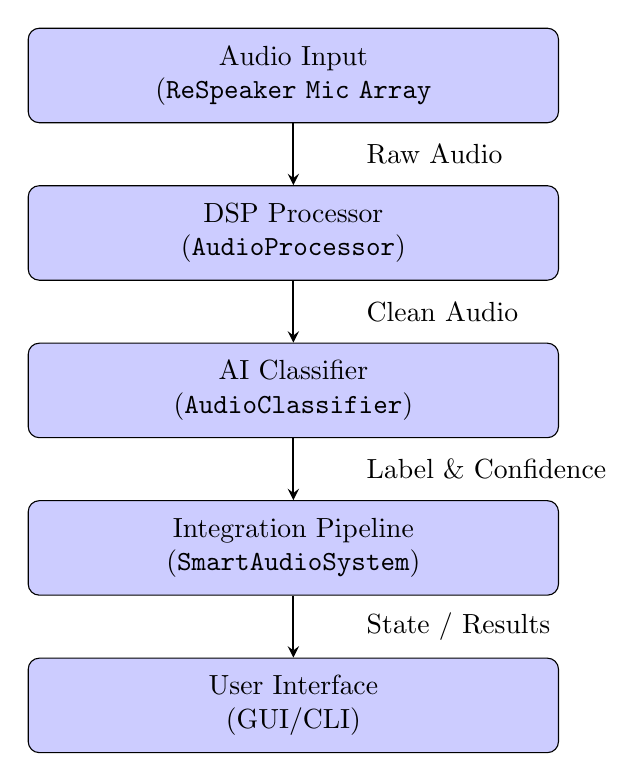
\begin{tikzpicture}[
    node distance=2cm,
    block/.style={rectangle, draw, fill=blue!20, text width=6.5cm, text centered, rounded corners, minimum height=1.2cm},
    arrow/.style={->, >=stealth, thick}
]
    \node [block] (input) {Audio Input\\(\texttt{ReSpeaker Mic Array} };
    \node [block, below of=input] (dsp) {DSP Processor\\(\texttt{AudioProcessor})};
    \node [block, below of=dsp] (ai) {AI Classifier\\(\texttt{AudioClassifier})};
    \node [block, below of=ai] (pipeline) {Integration Pipeline\\(\texttt{SmartAudioSystem})};
    \node [block, below of=pipeline] (ui) {User Interface\\(GUI/CLI)};

    \draw [arrow] (input) -- (dsp) node[midway, right, xshift=8mm] {Raw Audio};
    \draw [arrow] (dsp) -- (ai) node[midway, right, xshift=8mm] {Clean Audio};
    \draw [arrow] (ai) -- (pipeline) node[midway, right, xshift=8mm] {Label \& Confidence};
    \draw [arrow] (pipeline) -- (ui) node[midway, right, xshift=8mm] {State / Results};
\end{tikzpicture}

\caption{Luồng xử lý tổng quan của hệ thống theo pipeline}
\label{fig:system_architecture}
\end{figure}


%--------------------------------------------------------
\subsection{Module phần cứng: SoundDetector (USB VAD/DOA)}
\subsubsection{Mô tả chức năng}
\texttt{SoundDetector} chịu trách nhiệm giao tiếp với ReSpeaker Mic Array v2.0 qua USB (control transfer) để truy xuất các tín hiệu/trạng thái đã được phần cứng xử lý sẵn. Các chức năng chính gồm:
\begin{itemize}
    \item \textbf{VAD (Voice Activity Detection)}: trạng thái phát hiện giọng nói do phần cứng cung cấp; có thể dùng để đánh dấu đoạn có tiếng nói hoặc hỗ trợ hiển thị.
    \item \textbf{DOA (Direction of Arrival)}: ước lượng hướng nguồn âm trong miền $0$--$359^\circ$, phục vụ quan sát trực quan (radar/compass) và debug hành vi thu âm.
    \item \textbf{Control/Status}: đọc/ghi một số tham số vận hành (tùy firmware) để kiểm tra trạng thái thiết bị hoặc hiệu chỉnh khi cần.
\end{itemize}

\subsubsection{Giao tiếp USB}
Module sử dụng thư viện \texttt{pyusb} để thực hiện control transfer. Ví dụ minh họa thao tác đọc tham số DOA từ thiết bị:

\begin{lstlisting}[language=Python, caption={Ví dụ đọc DOA bằng USB control transfer}, basicstyle=\ttfamily\footnotesize]
response = dev.ctrl_transfer(
    bmRequestType=0xC0,  # CTRL_IN | VENDOR | DEVICE
    bRequest=0x00,
    wValue=0,
    wIndex=21,           # DOA parameter ID (depends on firmware)
    data_or_wLength=8
)
direction = int.from_bytes(response, byteorder='little')
\end{lstlisting}

%--------------------------------------------------------
\subsection{Module DSP Processor: AudioProcessor}
\subsubsection{Mô tả chức năng}
\texttt{AudioProcessor} thực hiện tiền xử lý tín hiệu nhằm cải thiện chất lượng đầu vào cho mô hình AI. Trong thực tế, tín hiệu thu được từ microphone có thể bị nhiễu nền, biến thiên biên độ hoặc chứa thành phần tần số không hữu ích. Do đó, DSP được áp dụng để: (i) loại bỏ phần nhiễu ngoài dải quan tâm, (ii) giảm nhiễu nền và (iii) ổn định mức âm lượng để mô hình AI hoạt động nhất quán hơn.
Pipeline DSP trong hệ thống gồm ba bước chính:
\begin{enumerate}
    \item \textbf{Bandpass Filter}: giới hạn dải tần hữu ích (100--7500\,Hz) để giảm rumble tần thấp và hiss tần cao.
    \item \textbf{Spectral Gating}: giảm nhiễu nền trong miền tần số, giúp tăng tỉ lệ tín hiệu/nhiễu trong bối cảnh môi trường có noise.
    \item \textbf{AGC (Automatic Gain Control)}: ổn định biên độ (RMS) theo mục tiêu, đồng thời có ngưỡng gate để tránh khuếch đại nhiễu khi gần im lặng.
\end{enumerate}

\subsubsection{Pipeline xử lý}
Hình~\ref{fig:dsp_pipeline} minh họa thứ tự xử lý của pipeline DSP.

\begin{figure}[H]
\centering
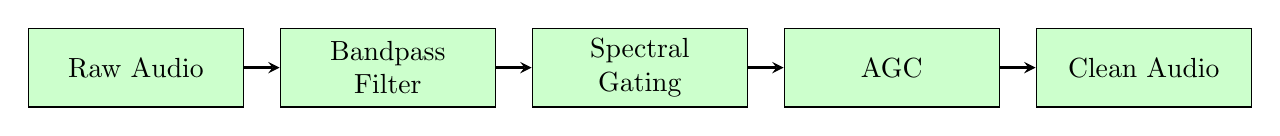
\begin{tikzpicture}[
    node distance=3.2cm,
    block/.style={rectangle, draw, fill=green!20, text width=2.5cm, text centered, minimum height=1cm},
    arrow/.style={->, >=stealth, thick}
]
    \node [block] (input) {Raw Audio};
    \node [block, right of=input] (bandpass) {Bandpass\\Filter};
    \node [block, right of=bandpass] (spectral) {Spectral\\Gating};
    \node [block, right of=spectral] (agc) {AGC};
    \node [block, right of=agc] (output) {Clean Audio};

    \draw [arrow] (input) -- (bandpass);
    \draw [arrow] (bandpass) -- (spectral);
    \draw [arrow] (spectral) -- (agc);
    \draw [arrow] (agc) -- (output);
\end{tikzpicture}
\caption{Pipeline xử lý DSP trước khi đưa tín hiệu vào mô hình AI.}
\label{fig:dsp_pipeline}
\end{figure}

%--------------------------------------------------------
\subsection{Module AI Classifier: AudioClassifier}
\subsubsection{Mô tả chức năng}
\texttt{AudioClassifier} thực hiện phân loại âm thanh môi trường theo hướng \textit{AI-only}. Về mặt luồng xử lý, module nhận \textit{clean audio} từ DSP và tạo ra kết quả dự đoán dạng \textit{label} và \textit{confidence}. Để mô hình hoạt động ổn định trong thời gian thực, hệ thống sử dụng các cơ chế theo thời gian (temporal logic) thay vì suy luận độc lập trên từng chunk nhỏ.

Các nhiệm vụ chính của module gồm:
\begin{itemize}
    \item \textbf{Feature Extraction}: chuyển tín hiệu audio đã qua DSP sang biểu diễn
    
    \textit{Log-Mel Spectrogram}.
    \item \textbf{Buffering/Windowing}: tích lũy dữ liệu theo cửa sổ ngắn (ví dụ vài giây) để tạo input đủ ``già'' cho mô hình.
    \item \textbf{Inference}: chạy mô hình CNN để dự đoán phân phối xác suất theo lớp, sau đó lấy nhãn top-1 và độ tin cậy.
    \item \textbf{Temporal Post-processing}: làm mượt dự đoán theo thời gian và xử lý trường hợp im lặng nhằm giảm jitter của nhãn.
\end{itemize}

\subsubsection{Post-processing và ổn định theo thời gian}
Để tăng độ ổn định dự đoán trong thời gian thực, hệ thống áp dụng các kỹ thuật sau:
\begin{itemize}
    \item \textbf{Smoothing}: trung bình hóa/xử lý tích lũy dự đoán trên $K$ bước gần nhất nhằm giảm nhảy nhãn do nhiễu hoặc dao động nhỏ của tín hiệu.
    \item \textbf{Confidence threshold}: nếu confidence dưới ngưỡng, hệ thống trả về \texttt{unknown} để hạn chế dự đoán ngẫu nhiên.
    \item \textbf{Fast-switch}: cho phép chuyển nhãn nhanh khi lớp mới có confidence cao và xuất hiện liên tiếp, giúp phản ứng tốt với sự kiện âm thanh rõ ràng.
    \item \textbf{Reset on silence}: khi RMS thấp liên tục vượt quá một khoảng thời gian, buffer/lịch sử sẽ được reset để tránh ``dính'' nhãn cũ.
\end{itemize}

%--------------------------------------------------------
\subsection{Module Integration Pipeline: SmartAudioSystem}
\subsubsection{Mô tả chức năng}
\texttt{SmartAudioSystem} đóng vai trò \textit{orchestrator}, kết nối các module xử lý (DSP) và suy luận (AI) thành một pipeline end-to-end. Module này chuẩn hóa đầu ra dưới dạng một \textit{state} thống nhất (ví dụ: RMS, gain, label, confidence), từ đó GUI và CLI chỉ cần đọc state để hiển thị mà không phụ thuộc vào chi tiết nội bộ của từng khối.

\subsubsection{Quản lý luồng xử lý}
Pipeline hoạt động theo vòng lặp liên tục:
\begin{enumerate}
    \item Thu audio theo chunk (ví dụ 1024 samples $\approx$ 64ms ở 16kHz).
    \item Tiền xử lý DSP (Bandpass $\rightarrow$ Spectral Gate $\rightarrow$ AGC).
    \item Cập nhật buffer/window và suy luận AI theo cơ chế \textit{hop} (không nhất thiết suy luận mỗi chunk).
    \item Đóng gói kết quả thành state kèm metadata (RMS, gain, label/confidence).
    \item Chuyển state đến tầng hiển thị (GUI/CLI).
\end{enumerate}

%--------------------------------------------------------
\subsection{Module User Interface}
\subsubsection{GUI}
GUI được xây dựng bằng Tkinter theo mô hình đa luồng để đảm bảo giao diện luôn responsive. Do Tkinter không thread-safe, toàn bộ cập nhật UI chỉ thực hiện trên main thread. Worker thread đảm nhiệm chạy pipeline và đẩy state sang main thread thông qua queue an toàn luồng (Hình~\ref{fig:gui_threading}).

\begin{figure}[H]
\centering
\begin{tikzpicture}[
    block/.style={
        rectangle, draw, fill=orange!20,
        text width=4.2cm, text centered,
        minimum height=1.2cm
    },
    arrow/.style={->, >=stealth, thick}
]
    \node[block] (main) {Main Thread\\(UI Updates)};
    \node[block, below=1.4cm of main] (queue) {Queue\\(Thread-safe)};
    \node[block, below=1.4cm of queue] (worker) {Worker Thread\\(Audio Pipeline)};

    % Worker -> Queue (put)
    \draw[arrow] (worker.north) -- node[right]{\small put()} (queue.south);

    % Queue -> Main (get)
    \draw[arrow] (queue.north) -- node[right]{\small get()} (main.south);
\end{tikzpicture}
\caption{Mô hình threading cho GUI}
\label{fig:gui_threading}
\end{figure}


\noindent\textbf{Các thành phần giao diện} có thể bao gồm:
\begin{itemize}
    \item \textbf{DSP Panel}: hiển thị RMS đầu vào/đầu ra và hệ số gain của AGC.
    \item \textbf{AI Panel}: hiển thị nhãn dự đoán và confidence.
    \item \textbf{Radar/Direction Panel (tuỳ chọn)}: hiển thị DOA nếu bật \texttt{SoundDetector}.
    \item \textbf{Event Logs}: lưu các sự kiện theo thời gian để quan sát hành vi hệ thống.
\end{itemize}

\subsubsection{CLI}
CLI được xây dựng bằng thư viện Rich nhằm hỗ trợ kiểm thử nhanh và theo dõi realtime. CLI được thiết kế như một tầng mỏng (thin layer), tái sử dụng cùng pipeline với GUI để đảm bảo đầu ra nhất quán, đồng thời hỗ trợ quan sát nhanh các chỉ số quan trọng (RMS/gain/label/confidence) mà không cần chạy giao diện đồ họa.

\pagebreak
%========================================================
% Implementation
%========================================================
\section{Implementation}

\subsection{Cấu trúc mã nguồn}

\subsubsection{Tổng quan tổ chức code}
Hệ thống được tổ chức theo cấu trúc modular, trong đó mỗi module đảm nhận một trách nhiệm cụ thể. Cấu trúc thư mục được thiết kế để tối ưu hóa khả năng bảo trì, mở rộng và tái sử dụng code.

\begin{lstlisting}[caption={Cấu trúc thư mục dự án}, basicstyle=\ttfamily\footnotesize, frame=single]
Sound-detect-Service/
|
+-- Core Components:
|   +-- audio_classifier.py
|   +-- audio_processor.py 
|   +-- sound_detector.py  
|   +-- smart_audio_pipeline.py 
|
+-- User Interface:
|   +-- gui_app.py 
|   +-- cli.py
|
+-- Configuration:
|   +-- config.py
|
+-- AI Model:
    +-- audio_cnn_best.h5 (14 classes)
    +-- audio_classifier_model.ipynb
\end{lstlisting}

\subsubsection{Chi tiết các module chính}
Bảng~\ref{tab:code_structure} mô tả chi tiết chức năng của từng file trong hệ thống.

\begin{table}[H]
\centering
\small
\begin{tabular}{|l|p{8.5cm}|}
\hline
\textbf{File} & \textbf{Chức năng} \\ \hline
\texttt{sound\_detector.py}  & Giao tiếp USB với ReSpeaker, đọc VAD/DOA, 

quản lý kết nối hardware \\ \hline
\texttt{audio\_processor.py} & DSP pipeline: Bandpass Filter, Spectral Gating, AGC với stateful processing \\ \hline
\texttt{audio\_classifier.py}  & AI classifier: Feature extraction,

CNN inference, temporal smoothing, buffering \\ \hline
\texttt{smart\_audio\_pipeline.py}  & Integration orchestrator: kết nối DSP + AI, chuẩn hóa output, lifecycle management \\ \hline
\texttt{gui\_app.py} & Tkinter GUI với threading model, 

queue-based communication, real-time visualization \\ \hline
\texttt{cli.py} & Rich CLI với commands (start, status, test), 

terminal-based monitoring \\ \hline
\texttt{config.py}  & Configuration constants: thresholds, paths, 

hyperparameters \\ \hline
\end{tabular}
\caption{Chi tiết các module chính trong hệ thống}
\label{tab:code_structure}
\end{table}

% \subsection{Pipeline tích hợp trong \texttt{smart\_audio\_pipeline.py}}
% File \texttt{smart\_audio\_pipeline.py} định nghĩa lớp \texttt{SmartAudioSystem} như một lớp \textit{orchestrator}, có nhiệm vụ ghép toàn bộ chuỗi xử lý thời gian thực thành một API đơn giản: \textit{mỗi vòng lặp đọc một chunk âm thanh, xử lý, dự đoán, rồi trả về một kết quả chuẩn hóa}. Thiết kế này giúp GUI/CLI không phải gọi trực tiếp vào các hàm nội bộ của DSP hay AI, từ đó giảm coupling và giảm nguy cơ mismatch khi thay đổi module.

% \subsubsection{API chính của \texttt{SmartAudioSystem}}
% Ở mức code, \texttt{SmartAudioSystem} thường cung cấp các nhóm hàm sau:
% \begin{itemize}
%     \item \textbf{Khởi tạo và cấu hình}: tạo đối tượng \texttt{AudioProcessor} và \texttt{AudioClassifier}, đọc tham số từ \texttt{config.py} (sample rate, chunk size, hop/window,\ldots).
%     \item \textbf{Vòng xử lý 1 bước}: hàm \texttt{process\_and\_predict()} thực hiện toàn bộ pipeline cho một chunk và trả về state.
%     \item \textbf{Vòng chạy liên tục}: GUI/CLI gọi \texttt{process\_and\_predict()} lặp lại trong worker loop (GUI) hoặc loop console (CLI).
% \end{itemize}

% \subsubsection{Luồng xử lý trong \texttt{process\_and\_predict()}}
% Luồng xử lý của hàm \texttt{process\_and\_predict()} có thể mô tả theo các bước tương ứng với code như sau:
% \begin{enumerate}
%     \item \textbf{Đọc âm thanh thô}: gọi \texttt{read\_audio\_chunk()} từ \texttt{AudioClassifier} (module này quản lý audio stream) để lấy \texttt{raw\_chunk}. Nếu không đọc được (stream lỗi hoặc đang dừng), hàm trả về \texttt{None} để tầng gọi xử lý.
%     \item \textbf{Tiền xử lý DSP}: đưa \texttt{raw\_chunk} qua \texttt{AudioProcessor.process()} để thu được \texttt{clean\_chunk} và cập nhật các chỉ số như RMS/gain.
%     \item \textbf{Suy luận AI}: truyền \texttt{clean\_chunk} vào \texttt{AudioClassifier.classify\_chunk()} để nhận \texttt{env\_label}, \texttt{env\_conf} và các chỉ số liên quan (ví dụ RMS sau xử lý).
%     \item \textbf{Chuẩn hóa đầu ra}: đóng gói kết quả thành một \textit{state} dạng dictionary để GUI/CLI sử dụng thống nhất.
% \end{enumerate}

% \subsubsection{Định dạng \textit{state} trả về}
% Đầu ra của pipeline được chuẩn hóa để phục vụ hiển thị và logging. Một state điển hình bao gồm:
% \begin{itemize}
%     \item \textbf{Kết quả AI}: \texttt{env\_label} (nhãn top-1) và \texttt{env\_conf} (độ tin cậy).
%     \item \textbf{Chỉ số DSP}: \texttt{rms\_raw}, \texttt{rms\_clean}, \texttt{gain\_applied} (giúp quan sát hiệu ứng của tiền xử lý).
%     \item \textbf{Trạng thái bổ sung (tuỳ chọn)}: \texttt{timestamp} hoặc \texttt{frame\_index} để đồng bộ UI/log.
% \end{itemize}

% \subsubsection{Cơ chế chạy realtime và dừng/chạy lại an toàn (mức code)}
% Trong GUI, pipeline chạy trong worker thread để tránh chặn main thread. Cơ chế an toàn khi chạy/dừng thường dựa trên hai nguyên tắc:
% \begin{itemize}
%     \item \textbf{Stop flag / stop event}: worker loop kiểm tra cờ dừng mỗi iteration; khi người dùng bấm Stop, cờ được set để worker thoát vòng lặp một cách ``graceful''.
%     \item \textbf{Cleanup tài nguyên theo thứ tự}: khi thoát loop, hệ thống đóng audio stream (PyAudio), giải phóng handle của ReSpeaker (USB) nếu có, và đặt lại trạng thái nội bộ để cho phép Start lại.
% \end{itemize}

% \noindent Ở mức triển khai, worker loop (GUI) có dạng:
% \begin{itemize}
%     \item \textbf{while running}: gọi \texttt{process\_and\_predict()} $\rightarrow$ nhận state $\rightarrow$ \texttt{queue.put(state)}.
%     \item Main thread định kỳ lấy state mới nhất từ queue và cập nhật UI bằng \texttt{after()}.
% \end{itemize}

% \noindent Khi dừng, main thread set cờ dừng; worker thread hoàn tất iteration hiện tại, thực hiện cleanup và kết thúc. Cuối cùng, main thread có thể \texttt{join()} worker thread (với timeout) để đảm bảo không còn luồng nền nào giữ tài nguyên microphone, tránh lỗi khi Start lại ngay lập tức.












%--------------------------------------------------------
\subsection{Pipeline tích hợp trong \texttt{smart\_audio\_pipeline.py}}

File \texttt{smart\_audio\_pipeline.py} định nghĩa lớp \texttt{SmartAudioSystem} như một lớp 

\textit{orchestrator}, có nhiệm vụ ghép chuỗi xử lý thời gian thực thành một API thống nhất.

Mỗi lần gọi, hệ thống đọc một chunk âm thanh, chạy DSP, suy luận AI và trả về một \textit{state} chuẩn hóa. 

Nhờ đó, GUI/CLI chỉ làm nhiệm vụ hiển thị và điều khiển, không cần phụ thuộc vào chi tiết nội bộ của DSP/AI.

\subsubsection{Luồng xử lý trong \texttt{process\_and\_predict()}}
Hình~\ref{fig:pipeline_flow} minh họa luồng xử lý chính của hàm \texttt{process\_and\_predict()}.

\begin{figure}[!t]
\centering
\resizebox{0.78\linewidth}{!}{%
\begin{tikzpicture}[
    node distance=1.3  cm,
    process/.style={
        rectangle, draw,
        fill=blue!15,
        text width=4.8cm,
        align=center,
        minimum height=1.1cm,
        rounded corners,
        font=\small
    },
    decision/.style={
        diamond, draw,
        fill=yellow!15,
        align=center,
        inner sep=1pt,
        font=\small,
        minimum size=1.4cm,  % <<< quan trọng: tăng kích thước diamond
        aspect=2.8            % <<< làm diamond "bè" ra để chứa chữ
    },
    ret/.style={
        rectangle, draw,
        fill=green!15,
        text width=4.2cm,
        align=center,
        minimum height=1.0cm,
        rounded corners,
        font=\small
    },
    arrow/.style={->, >=stealth, thick}
]
    % Nodes
    \node[process] (read) {Read Audio Chunk\\(\texttt{read\_audio\_chunk()})};
    \node[decision, below=0.95cm of read] (valid) {Valid?}; % <<< giờ sẽ không tràn
    \node[process, below=0.95cm of valid] (dsp) {DSP Processing\\(\texttt{processor.process()})};
    \node[process, below=0.95cm of dsp] (ai) {AI Inference\\(\texttt{classifier.classify\_chunk()})};
    \node[ret, below=0.95cm of ai] (state) {Return State\\(\texttt{dict})};

    \node[ret, right=4.2cm of valid] (none) {Return None};

    % Arrows
    \draw[arrow] (read) -- (valid);
    \draw[arrow] (valid) -- node[left, font=\scriptsize] {Yes} (dsp);
    \draw[arrow] (dsp) -- (ai);
    \draw[arrow] (ai) -- (state);

    \draw[arrow] (valid) -- node[above, font=\scriptsize] {No} (none);
\end{tikzpicture}%
}
\caption{Luồng xử lý trong hàm \texttt{process\_and\_predict()}.}
\label{fig:pipeline_flow}
\end{figure}



\noindent Luồng xử lý có thể tóm tắt như sau:
\begin{enumerate}
    \item \textbf{Đọc chunk}: lấy \texttt{raw\_chunk} từ audio stream. Nếu không có dữ liệu hợp lệ, trả về \texttt{None}.
    \item \textbf{DSP}: xử lý \texttt{raw\_chunk} để tạo \texttt{clean\_chunk} và 
    
    cập nhật một số chỉ số giám sát (RMS/gain).
    \item \textbf{AI}: suy luận trên \texttt{clean\_chunk} và tạo kết quả \texttt{label/confidence}
    
    (có thể chạy theo cơ chế hop/window).
    \item \textbf{Đóng gói}: chuẩn hóa đầu ra thành state cho GUI/CLI.
\end{enumerate}

\subsubsection{Pseudo-code triển khai}
Listing~\ref{lst:process_predict} minh họa pseudo-code của \texttt{process\_and\_predict()} (các chi tiết DSP/AI được trình bày ở các phần sau của báo cáo).

\begin{lstlisting}[language=Python, caption={Pseudo-code: \texttt{process\_and\_predict()}}, label={lst:process_predict}, basicstyle=\ttfamily\footnotesize, frame=single]
def process_and_predict(self):
    raw_chunk = classifier.read_audio_chunk()
    if raw_chunk is None:
        return None

    clean_chunk = processor.process(raw_chunk)
    env_label, env_conf, rms_clean = classifier.classify_chunk(clean_chunk)

    return {
        "env_label": env_label,
        "env_conf": float(env_conf),
        "rms_raw": float(rms(raw_chunk)),
        "rms_clean": float(rms_clean),
        "gain_applied": float(processor.current_gain),
        # optional: timestamp / frame_index
    }
\end{lstlisting}

\subsubsection{Định dạng \textit{state} trả về}
Đầu ra của pipeline được chuẩn hóa thành dictionary với các trường chính như Bảng~\ref{tab:state_format}.

\begin{table}[H]
\centering
\begin{tabular}{|l|l|p{5.4cm}|}
\hline
\textbf{Field} & \textbf{Type} & \textbf{Mô tả} \\ \hline
\texttt{env\_label} & str/None & Nhãn dự đoán; có thể 

\texttt{None}/\texttt{unknown} 

tùy logic realtime \\ \hline
\texttt{env\_conf} & float & Độ tin cậy (0--1) \\ \hline
\texttt{rms\_raw} & float & RMS của audio đầu vào \\ \hline
\texttt{rms\_clean} & float & RMS sau tiền xử lý DSP \\ \hline
\texttt{gain\_applied} & float & Gain hiện tại do AGC áp dụng \\ \hline
\end{tabular}
\caption{Định dạng state dictionary trả về từ pipeline.}
\label{tab:state_format}
\end{table}

\subsubsection{Cơ chế realtime trong GUI (thread + queue)}
Hình~\ref{fig:realtime_mechanism} mô tả cơ chế chạy realtime: worker thread liên tục tạo state và đẩy vào queue; main thread định kỳ lấy state (ưu tiên state mới nhất) để cập nhật UI an toàn.


\begin{figure}[H]
\centering
\begin{tikzpicture}[
    node distance=1.5cm and 3cm,
    block/.style={rectangle, draw, fill=orange!15, text width=3cm, text centered, minimum height=1cm, font=\small},
    loop/.style={rectangle, draw, fill=cyan!15, text width=3.5cm, text centered, minimum height=1.2cm, font=\small},
    arrow/.style={->, >=stealth, thick}
]
    % Worker Thread
    \node [loop] (worker) {\textbf{Worker Thread}\\Audio Processing Loop};
    \node [block, below=of worker] (process) {process\_and\_\\predict()};
    \node [block, below=of process] (put) {queue.put(state)};
    
    % Queue
    \node [block, right=of process] (queue) {\textbf{Queue}\\(Thread-safe)};
    
    % Main Thread  
    \node [loop, right=of queue] (main) {\textbf{Main Thread}\\UI Update Loop};
    \node [block, below=of main] (get) {queue.get()};
    \node [block, below=of get] (update) {Update UI};
    
    % Arrows
    \draw [arrow] (worker) -- (process);
    \draw [arrow] (process) -- (put);
    \draw [arrow] (put) -| (queue);
    \draw [arrow] (queue) |- (get);
    \draw [arrow] (get) -- (update);
    
    % Loop arrows
    \draw [arrow, dashed] (put.west) -- ++(-0.8,0) |- (worker.west);
    \draw [arrow, dashed] (update.east) -- ++(0.8,0) |- (main.east);
    
    % Labels
    \node [above=0.2cm of worker, font=\scriptsize] {while is\_running:};
    \node [above=0.2cm of main, font=\scriptsize] {root.after(50ms)};
\end{tikzpicture}
\caption{Cơ chế realtime với worker thread và queue}
\label{fig:realtime_mechanism}
\end{figure}
\FloatBarrier


\subsubsection{Dừng/chạy lại an toàn}
Để tránh rò rỉ tài nguyên và đảm bảo có thể Start/Stop nhiều lần, hệ thống sử dụng cơ chế \textit{stop flag/stop event} cho worker loop và thực hiện cleanup theo thứ tự. Khi Stop, main thread gửi tín hiệu dừng; worker thread thoát vòng lặp một cách graceful và đóng audio stream/giải phóng tài nguyên. Khi Start lại, hệ thống khởi tạo lại các thành phần cần thiết và khởi chạy worker thread mới với trạng thái sạch.
